\documentclass{beamer}


\graphicspath{ {images/} }

\usetheme{Boadilla}

\title{Spotting Distracted Drivers}
\subtitle{HLCV Project}
\author[Reyes, Schaefer, Tonsen, Weber]{Guillermo Reyes \\
	 Daniel Schaefer \\
	 Marc Tonsen \\
 Dominik Weber\\}
 \institute[]{Saarland University}
\date{20.06.2016}



\begin{document}
	\begin{frame}
		\titlepage
	\end{frame}
	
	\begin{frame}
		\frametitle{Outline}
		\tableofcontents
	\end{frame}
	
	\section{Task and Motivation}	
	\begin{frame}
		\frametitle{Task}
		\only<1>{We will enter a Computer Vision Competition: State Farm Distracted Driver Detection. We are given pictures of several drivers doing different activities, the  goal is to predict the likelihood of what the driver is doing in each picture.
		\begin{itemize}
			\item c0 safe driving
			\item c1: texting - right
			\item c2: talking on the phone - right
			\item c3: texting - left
			\item c4: talking on the phone - left
			\item c5: operating the radio
			\item c6: drinking
			\item c7: reaching behind
			\item c8: hair and makeup
			\item c9: talking to passenger			
		\end{itemize}}
		\begin{onlyenv}<2-10>
			\begin{center}
				\includegraphics<2>[scale = .4]{img_0}
				\includegraphics<3>[scale = .4]{img_5}
				\includegraphics<4>[scale = .4]{img_6}
				\includegraphics<5>[scale = .4]{img_14}
				\includegraphics<6>[scale = .4]{img_19}
				\includegraphics<7>[scale = .4]{img_26}
				\includegraphics<8>[scale = .4]{img_34}
				\includegraphics<9>[scale = .4]{img_56}
				\includegraphics<10>[scale = .4]{img_94}
				
			\end{center}
			content...
		\end{onlyenv}
	\end{frame}
	
	\begin{frame}
		\frametitle{Motivation}
		According to the national Highway Traffic Safety Administration, about ten percent of fatal crashes, 18 percent of injury crashes, and
		16 percent of all police-reported motor vehicle traffic crashes
		every year are reported as distraction-affected crashes. This translates to over 3000 people killed and over 400,000 injured in motor vehicle crashes involving driver distraction in the US alone.
		
		It is thus, imperative to take measures regarding distracted drivers, starting by being able to detect them. Unfortunately using specialized sensors and trackers would be really expensive, but simple cameras are more affordable and could be installed in a non-intrusive way in the vehicles, then with the help of computer vision techniques distracted drivers could be identified and appropriate measures could then be taken
	\end{frame}
	
	\begin{frame}
		\frametitle{Related Work}
		Different approaches have been taken to deal with this problem. In \cite{Ragab2014} driving sessions of 6 different drivers were recorded with infrared and kinect cameras in front of the drivers, and used different classifiers such as SVMs Random Forests and HMMs to determine the activity performed by the subject and achieved up to 82\% accuracy on these 6 subjects. 
		
		
		\begin{figure}
			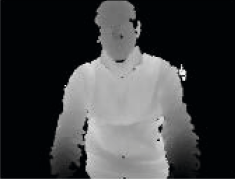
\includegraphics{RanFor}
			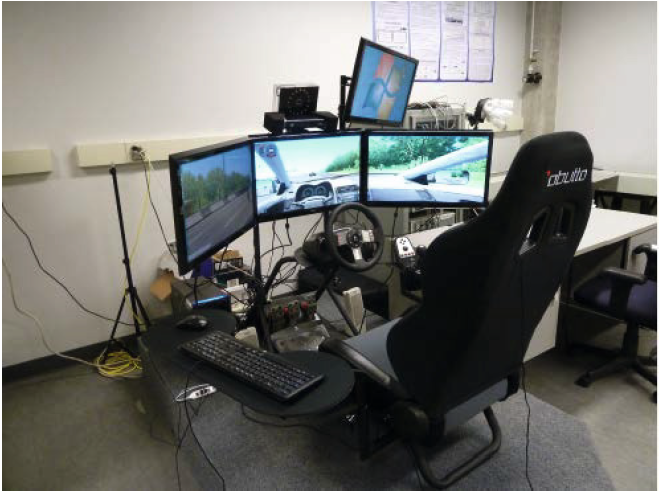
\includegraphics[scale = .365]{RanForSim}
		\end{figure}
		\begin{figure}
			
			
			
		\end{figure}
	\end{frame}
	
	
	%{\begin{frame}
%		\frametitle{Related Work}
%		Some approaches have been taken using computer vision to determine the inattention level of driver by looking at the face 
%		
		
%		\begin{figure}
%			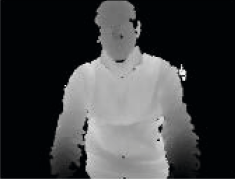
\includegraphics{RanFor}
%			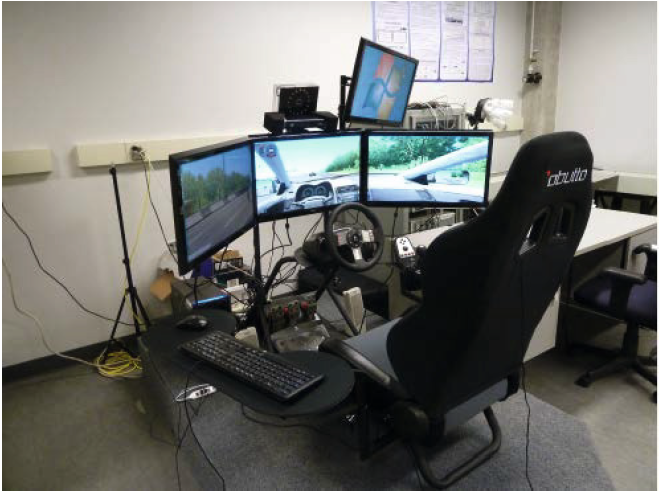
\includegraphics[scale = .365]{RanForSim}
%		\end{figure}
%		\begin{figure}
			
			
			
%		\end{figure}
%	\end{frame}
	
	\section{Modls Tools, Novelty}	

    \begin{frame}
        \frametitle{Tentative Material and Methods}
        \begin{itemize}
            \item Support Vector Machines (based on SIFT and HOG features)
            \item Random Forests
            \item using Matlab
            \item AlexNet in Caffe
        \end{itemize}

    \end{frame}

    \begin{frame}
		\frametitle{Investigation}
        \begin{center}
        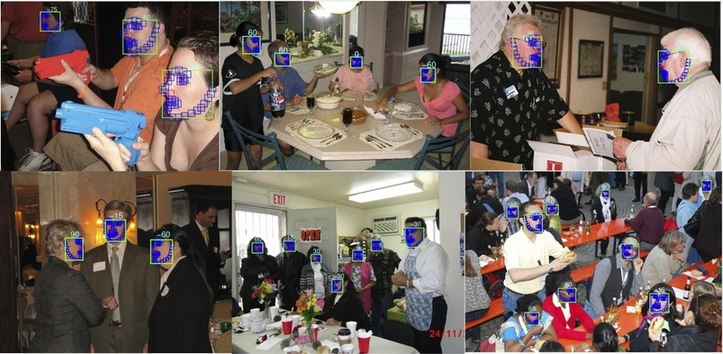
\includegraphics[width=10cm]{images/FacePose.jpg}\\
        Face pose detection using existing algorithms\end{center}
    \end{frame}

    \begin{frame}
		\frametitle{Investigation}
        \begin{center}
        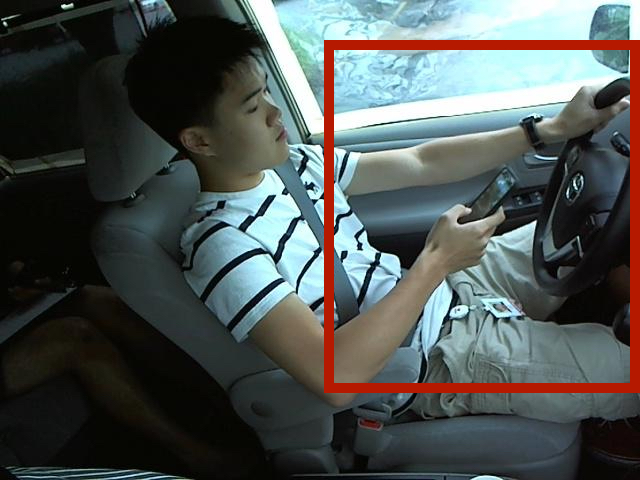
\includegraphics[width=9cm]{images/HandLocalisation.jpg}\\
        Rough classification in vicinity of the steering wheel using a hard-coded cropped version of our picture\end{center}
    \end{frame}


    \begin{frame}
		\frametitle{Investigation}
        \begin{center}
        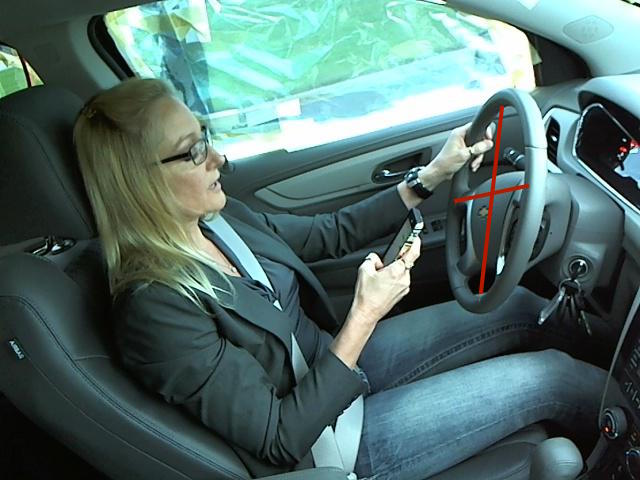
\includegraphics[width=9cm]{images/CameraPose.jpg}\\
        Camera-pose estimation using the steering-wheel pose\end{center}
    \end{frame}


    \begin{frame}
		\frametitle{Investigation}
        \begin{center}
        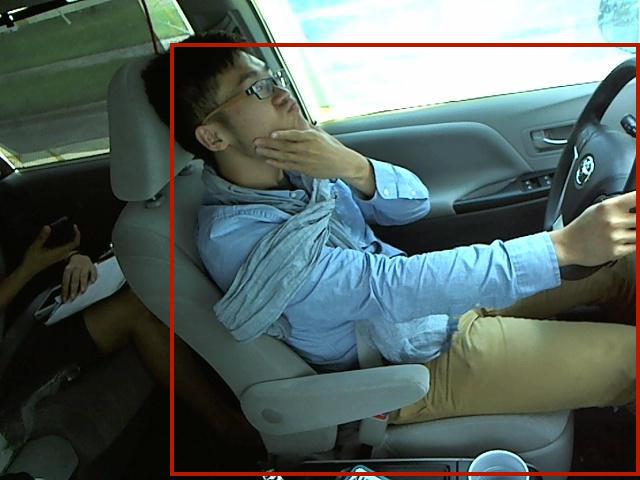
\includegraphics[width=9cm]{images/BoundingBox.jpg}\\
        Estimating Bounding-Box surrounding the driver to reduce search space potentially using the detected face and steering-wheel pose\end{center}
    \end{frame}

	
	\section{Analysis}	
	\begin{frame}
		\frametitle{Benchmark}
		Over 22000 images are provided as training set by the competition as well as a list with the labels. The train and test data are split on the drivers, such that one driver can only appear on either train or test set. 		


	\end{frame}

		
		


		
		\begin{frame}[allowframebreaks]
			\frametitle{References} 
			\nocite{*} 
			\bibliographystyle{amsalpha} 
			\bibliography{references} 
		\end{frame}
		
		\medskip	
		

	
		

\end{document}
